\chapter{if conversion \Author{C. Bruel}}
\inputprogress
\graphicspath{{img/}{if_conversion/img/}{part4/if_conversion/img/}}
	
\newcommand\cond{~?~}

\setcounter{tocdepth}{3} 
\tableofcontents

\section{Overview/Motivations}

We describe in this chapter an if-conversion framework in SSA, that allows to transform a regions of basic blocks into an a region were branches have been removed and instructions transformed into a conditional representation by the target architecture.

\subsection{Introduction}

One way to increase the instruction throughput is to increase the number of instructions that can be issued simultaneously. In order to fully exploit the parallelism made available by multiple issues processors \cite{Rau:2003:IP:1074100.1074489}, Instruction Level Parallelism techniques are implemented in the hardware, such as-out-of-order execution, or dynamic scheduling, branch prediction. However, a more economical trend delegates to the compiler the task to extract and organize ILP thu the envent of Explicitly scheduled architectures, such as EPIC (Explicitly Parallel Architectures), or VLIW (Very Large Instruction World).

Conditional branches introduce control dependencies between instructions. An instruction is control dependent on a preceding instruction if the first one determines the execution of the second one \cite{Kennedy:2001:OCM:502981}. They limit the scope of ILP optimizations, because they reduce the number of continuous instructions that are not data dependent and thus can be executed in parallel. By reducing the average size of a basic block, they act as a bottleneck for exposing parallelism.

If-conversion is the process of transforming a control flow region containing a several basic blocks into a single basic block of straight line of conditional instructions. Thus removing control branches from this region \cite{Schlansker97achievinghigh}. The conditional instructions are implemented on the target machine using the predication or speculation techniques described bellow.

Removing branches improves performance in several ways: by removing the mis-prediction penalty, the instruction fetch throughput is increased and the instruction cache miss penalty reduced. Enlarging the size of the basic blocks allows the static scheduler to schedule earlier long latencies operations and to improve the ILP by merging multiple control paths into a single flows of execution. Many compiler optimizations are impacted by branches. Software Pipelining for example, can't efficiently schedule loops with conditional branches \cite{Warter:1992:EMS:144953.145796}.

Consider \ref{fig:example1}, that represents the execution of a simple if-then-else statement on a hypothetical 3-issue processor. Branches are not highly biased, so the schedule height is 4 instructions, and 2 branches.

\begin{figure}
  \centering
  \subfigure[Control Flow] {
    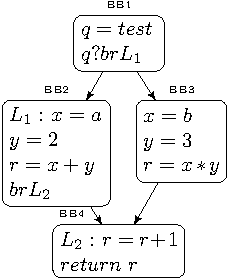
\includegraphics[scale=0.8]{specul.pdf}
    \label{fig:orig}}
  \subtable[Speculated] {
    \begin{tabular}{|l|l|l|}
      $q = test$ & $p = test$ & $y1=b$  \\
      $x1=a$ & $x2=2$ & $y2=3$  \\
      $x=q?x1:x2$ & $y=p?y1:y2$ \\
    \end{tabular}
    \label{fig:specul}}
  \subtable[Afer propagation] {
    \begin{tabular}{|l|l|l|}
      $q = test$ & $p = test$ &  \\
      $x=q?a:2$ & $y=p?b:3$ & \\
    \end{tabular}
    \label{fig:specul2}}
  \subtable[Predicated] {
    \begin{tabular}{|l|l|l|}
      $q = test$ & $p=test$ &  \\
      $q?x=a$ & $\bar{q}?x=3$ &  \\
      $p?y=b$ & $\bar{p}?y=2$ &  \\
    \end{tabular}
    \label{fig:predil}}
\caption{Benefit example}
\label{fig:example1}
\end{figure}

After if-conversion the execution path is reduced to 2 cycles. We can observe that if-conversion implied 2 optimisations.
\begin{itemize}
\item  Merge of execution paths into a single execution path, which is even more beneficial when branch bredication is not availale, because of a better exploitation of available resources.  
\item Reduction of the schedule length, because instructions can be speculated before the branch.
\end{itemize}

\begin{itemize}
\item variables have been renamed, 
\item a \textit{merge} pseudo operation have been introduced. It is necessary to reconstruct the original value of $x$ and $y$.
\item This \textit{merge} introdudess a data dependency. if-conversion transforms control dependencies into data dependencies \cite{Allen:1983:CCD:567067.567085}. The first consequence is that all registers now live simultaneously, (live range), so the benefits of branch removing and better schedule balanced with increased live range and register pressure : If-conversion must rely on a powerfull decision model
\item. Works well with scalar optimizations, such as constant propagation in this example.
\end{itemize}

\subsection{Architectural requirements}
The example above shows that if-conversion we produce different code, based on the architectural features. The algorithm expect the architecture to provide support for conditional execution of instructions, or to conditionaly commit the result of an instruction.
Basically, two kind of support can (co-)exist: predicated execution or speculaive execution my mean of conditional moves. The latter is sometimes referenced as ``partial predication''

Predication \ref{fig:pred} is an architectural features that allows an instruction to be executed conditionally my mean of a predicate (for pipelined architectured, the instruction is always executed, but the results is nullified). 

\begin{figure}
\begin{minipage}[t]{4cm}
\mbox{fully predicated:} \\
$ p \cond x = a + b $ \\
$ \overline{p} \cond x = 0 $ \\
\end{minipage}
\begin{minipage}[t]{4cm}
\mbox{partially predicated:} \\
$t = a + b $ \\
$p \cond x = t $ \\
$\overline{p} \cond x = 0 $ \\
\end{minipage}
\label{fig:pred}
\end{figure}

Speculation \ref{fig:spec} is a compiler technique that allows an instruction to be executed unconditionnally. The result can be commited only when the condition is known to be true.

Those architectures must provide a instruction to commit the speculated value. select or conditional moves. Examples of conditional moves: cmov (Pentium Pro), select (ST 231 VLIW).

\begin{figure}
\begin{minipage}[t]{4cm}
\mbox{$cmov$ instruction:} \\
$t = a + b $ \\
$x = 0 $ \\
$x = cmoveq t $ \\
\end{minipage}
\begin{minipage}[t]{4cm}
\mbox{$select$ instruction:} \\
$t = a + b $ \\
$x = select p \cond t : 0 $ \\
\end{minipage}
\label{fig:spec}
\end{figure}

To be speculated, an instruction should not create have any other side effets, or hazards. For instance a memory load should not be able to trap (cache misses can also be considered for performance). 
Memory load operations can sometimes be speculated with architectural supports to dismiss potential bad memory access errors. Speculative load is important, because as a long latency operations, the data can be loaded far before it is really needed. 

\begin{figure}
\begin{minipage}[t]{4cm}
\mbox{speculative load:} \\
$t = ldw.d(addr) $ \\
$x = select p \cond t : 0 $ \\
\end{minipage}
\begin{minipage}[t]{4cm}
\mbox{speculative store} \\
$x=select p \cond addr : dummy $ \\
$stw (x, value) $
\end{minipage}
\label{fig:spec}
\end{figure}

The condition code must be visible at the ISA level, to enable boolean optimisation of predicates.

\section{SSA if-conversion}

SSA provides an efficient intermediate representation in which false data dependencies have been removed, removing the need for register renaming needed when merging two definitions into one. Each assignment target (def) is assigned a unique register name. Registers are re-materialized at join nodes using $\phi$ operations. A procedure is in minimal SSA form if the number of $\phi$ instructions at join nodes is as small as possible. In relation to the if-conversion, SSA-form representation ensure that a variable is assigned only once, and their merging point is exposed info $\phi$ operations.

\begin{figure}
\centering
    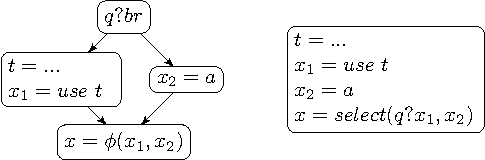
\includegraphics[scale=0.8]{ssa.pdf}
\caption{register selection}
\label{fig:ssa1}
\end{figure}

\begin{itemize}
\item Multiple definitions of a different variables assignment merged into a single path. This is inherently fixed in SSA, alleviating the need for renaming.
\item Minimize the number of instructions to be predicated. Only instruction that merge need to be conditionalized inside the predicate set that control the merge. Others can be safely executed when they don't produce hazard. For example in \ref{fig:ssa1}, only $x$ depends on the condition, so $t$ can be emmited unconditionally
\item Predicate assignments. Each instruction in the basic block that merge into the $\phi$ must be assigned to their defining predicate
\end {itemize}

Finally instructions must be emitted using speculation and conditional moves. in \ref{fig:nested1}, instructions from BB2 are assigned with the predicate $p$ and instructions from BB2 with the predicated $q\&t$. \ref{fig:nested2} shows the code layyout after predicate assignements. Then, In case of speculation execution model, predicated instructions have to be converted into conditional moves, using temporaries to hold arithmentic values. Additionally, a new predicate will need to be computed an assigned to each instruction.

\begin{figure}
\centering
  \subfigure[Nested test] {
    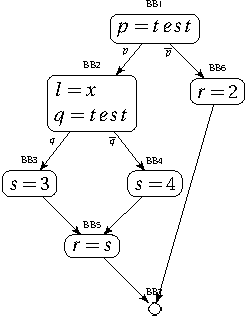
\includegraphics[scale=0.8]{nested1.pdf}
    \label{fig:nested1}}
  \subfigure[Predicate Assignments] {
    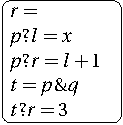
\includegraphics[scale=0.8]{nested2.pdf}
    \label{fig:nested2}}
  \subfigure[Conversion to speculated] {
    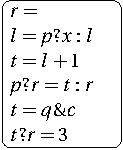
\includegraphics[scale=0.8]{nested3.pdf}
    \label{fig:nested}}
\caption{Traditional support for partial predication}
\label{fig:trad_part_pred}
\end{figure}

In contrast, consider the equivalent SSA if-conversion in \ref{fig:nest_ssa}, speculation is the genuine way of producing conditional moves out of $\phi$ instructions. Predicates don't need to be computed and temporaries values don't need to be conditionalized. As a result the SSA aggressive speculation technique produces a schedule length of 3. While traditional support produces in this case a schedule length of 4, without further expensive predicate reduction optimisation.

\begin{figure}
\centering
  \subfigure[Nested test] {
    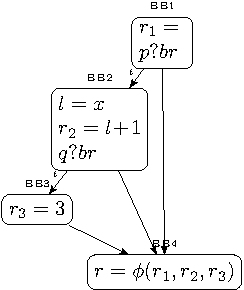
\includegraphics[scale=0.8]{nested4.pdf}
    \label{fig:nested4}}
  \subfigure[Inner if-conversion] {
    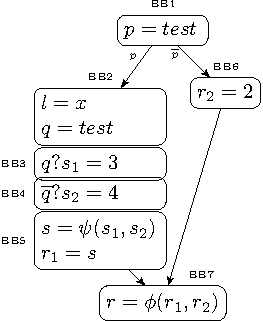
\includegraphics[scale=0.8]{nested5.pdf}
    \label{fig:nested5}}
  \subfigure[Global if-conversion] {
    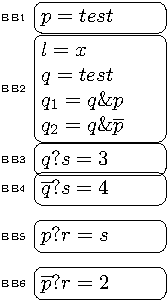
\includegraphics[scale=0.8]{nested6.pdf}
    \label{fig:nested6}}
\caption{Traditional partial predication}
\label{fig:nest_ssa}
\end{figure}

Note that basically, Since a SSA $\phi$ express the merging point of $n$ definitions from $n$ predecessors, the definition points depends on their nearest condition under which they depend. Intuitively we already know that thanks to SSA the definition point is straightforward to find, since it corresponds to the path by which the $\phi$ operand is reached. 
A very big difference is nature is the difference in the way the merging of conditional is realized using data dependencies instead of predicate selection. in SSA he condition merged assignment is not realized thru $\&$ if predicates, but by two successive conditional moves operations.

This algorithm takes as input SSA form and produces and produces a pure SSA using conditional move instructions to realize join points. One benefit of this approach is that all SSA properties are maintained, and scalar optimisations, such as constant propagation can be executed without predicate awareness..

\subsection{SSA operations on basic blocks}

SSA if-convertion works itratively from inner regions to outer regions, using a set of transformations on conditional branches that we describe here.

\begin{figure}
\begin{minipage}[t]{5cm}
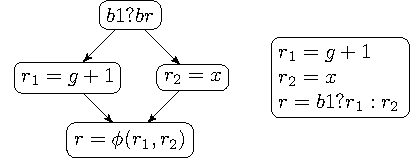
\includegraphics[scale=0.4]{phi_removal.pdf}
\caption{phi removal}
\label{fig:phi_rem}
\end{minipage}
\begin{minipage}[t]{5cm}
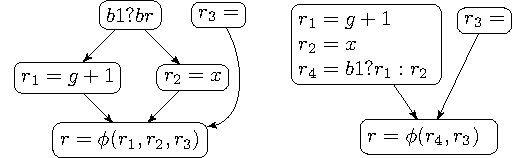
\includegraphics[scale=0.4]{phi_reduction.pdf}
\caption{phi reduction}
\label{fig:phi_red}
\end{minipage}
\begin{minipage}[t]{5cm}
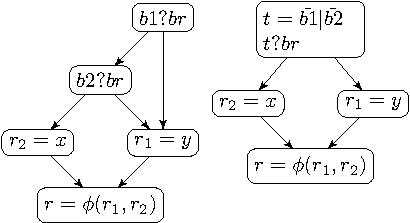
\includegraphics[scale=0.4]{phi_merge.pdf}
\caption{predicate merge}
\end{minipage}
\begin{minipage}[t]{5cm}
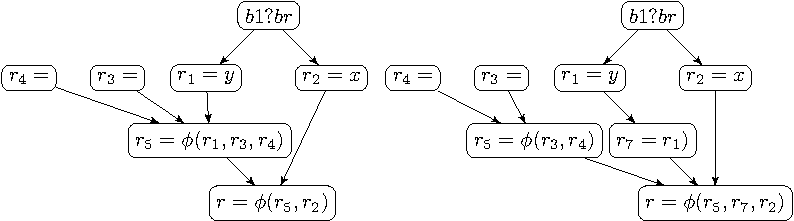
\includegraphics[scale=0.4]{phi_augmentation.pdf}
\caption{phi augmentation}
\label{fig:phi_aug}
\end{minipage}
\label{fig: phi_operations}
\end{figure}

The basic control structures that the analysis recognizes is the Single Exit region formed from the minimal set of blocks between a branch point and a merge point.  Those are minimal single entry single exit regions because at this point nested regions were already if-converted.

 We define this structure as the region between a conditional block and the first common immediate postdominator of the taken path block and the fall-thru block.

Note that each path can contain zero or more basic blocks with incoming edges.
As an optimization we allow two successive conditional blocks sharing one immediate post-dominator to be merged with logical operations after a normalization transformation. The normalization transformation ensures that conditional blocks sharing a same target can be merged by defining a wired $or$, or a wired $and$ share the same branch characteristics using branch reordering, test inversion or $de-morgan$ transformations.

\subsection{SSA representation of conditional instructions}

One problem of the described SSA-speculative framework is that it doesn't fit very well with a predicated model of conditional execution. Since $\phi$ are transformed to realize joint points into conditional moves, we should backwalk to relink the conditional moves into predicated instructions. This process of transforming speculation into predication is not convenient for many reasons:
- Predication introduces a renaming problem: Since a same register name can have 2 different assignments (under different predicates), this breaks SSA rules. The solution is to re-use the framework to realize join points into and extended SSA representation:el

In \ref{Stoutchinin:2001:ESS:563998.564022} $\psi$-SSA was described as a way to express a predicated form of SSA extension. Such representation is usually built from already predicated code, non SSA, originating from inlined assembly, peepholes, intrinsics functions or local transformations of control flow idioms. 

$\psi$-SSA expose the edge dependency from the basic block into which the definitionition of the $\phi$ argument is defined in the original CFG by a new data dependency. This dependency needs to be matemarialized into a $select$ or $\psi$ operation. Note that the $select$ operation is a real instruction that don't need to be replaced by the out-of-ssa process. If the target architecture doesn't provide such instruction to switch between speculated instruction, it can be emulated using two conditional moves. One advantage to generate $select$ instruction at this stage is that the program stays in full SSA form and make all the data dependencies explicit, and can be feed to all SSA optimizers. 

\begin{figure}
\begin{minipage}[t]{4cm}
\mbox{SSA:} \\
$ if (p) $ \\
$   x_1 = a+b $ \\
$ else $ \\
$   x_2 = 0 $ \\
$ x = \phi (x_1, x_2) $ \\
\end{minipage}
\begin{minipage}[t]{4cm}
\mbox{SSA-speculative form:} \\
$x_1 = a + b $ \\
$x_2 = 0 $ \\
$x = select p ? x_1, x_2$ \\
\end{minipage}
\begin{minipage}[t]{4cm}
\mbox{$\psi$-SSA form:} \\
$x_1 = a + b $ \\
$x_2 = 0 $\\
$x = \psi (p \cond x_1, \overline{p} x_2) $ \\
$y = \psi (p \cond x_1, \overline{p} x_2) $ \\
\end{minipage}
\end{figure}

Note that unlike $\phi$ arguments are executed simultaneously (they don't depend each other), $\psi$ arguments are executed sequentially and ordered from their definition predicate set. This propriety is necessary because if-conversion replaces the ``spacial'' dependency from the CFG by a ``temporal'' dependency from the straight line predicated code.

\subsection{SSA maintenance}

lConsider a conditional branch depending on a predicate $p$ and a region starting at $BBhead$. Let $BBp$ be the set of single exit basic blocks $(BBi,\dots,BB_n)$ that are on the taken path if $p$ is true and $BBq$ be the set of single exit basic blocks $(BBj,\dots,BB_m)$ that are executed if $p$ is false. The merge point of the if-converted region is at $BBjoin$. We distinct 4 types of basic SSA transformation that the framework uses and produces:
\subsubsection{$\phi$ removal} (figure \ref{fig:phi_rem})
The join node of the considered region has two predecessors and $\phi$ instructions are of the form $r=\phi(r_1,r_2)$. After speculation of the definitions of $r_1$ and $r_2$ the instruction can be rewritten as $r=\psi(p?r_1,\overline{p}?r_2)$.
\begin{proof} Once $BBp$ and $BBq$ have been promoted into $BBhead$, $BBjoin$ has for only predecessor $BBhead$ so it is not in its dominance frontier. The $\phi$ is not necessary and is removed.
\end{proof}
\subsubsection{$\phi$ reduction} (figure \ref{fig:phi_red})
 The join node of the considered region has $n$ predecessors that have $\phi$ instructions of the form $r=\phi(r_1,r_i,r_j,\dots,r_n)$. After merging, the $\phi$s are rewritten $t=\psi(p?r_i,\overline{p}?r_j)$ and a new $\phi$ $r=\phi(r_1,t,\dots,r_{n-1})$ is created with one operand less. The $\psi$ instruction is inserted after the speculated $r_i$ and $r_j$ definitions into $BBhead$.
\begin{proof} $BBjoin$ is still in the dominance frontier of $BBhead$, A $\phi$ must be redefined with the new definitions. The two corresponding $\phi$ edges from $BBq$ and $BBp$ can be replaced by the $BBhead$ edge.
The join block $E$ has $n$ predecessors with $n$ > 2, and $n$ blocks in its dominance frontier if it contains $\phi$s.
\end{proof}
\subsubsection{$\phi$ augmentation} (figure \ref{fig:phi_aug})
The objective is to remove incoming edges into the region. 
Consider a join node with $n$ predecessors among which $p$ is duplicated into $q$.  The join node of the considered region have $\phi$ instructions of the form $r=\phi(r_1,p,r_i,r_j,\dots,r_{n-1})$. The instruction is rewritten $t=select(p,r_i,r_j)$ and \mbox{$r=\phi(r_1,t,q,\dots,r_n)$}. 
\begin{proof}The duplicated blocks are new dominators of $BBjoin$ that define new $defs$. These blocks are now in the dominance frontier of $BBjoin$. SSA is maintained with new $\phi$ upgraded with the new reaching points.
Since the algorithm works the control flow in post order mode, the dominator tree doesn't change, and it's possible to maintain the SSA locally to the inner region. By recurence the if-converted region can be in turn be optimized out if it's head belongs to the dominance frontier of an outer region.
\end{proof}
Note that block duplication doesn't necessary implies more code size, since data flow dependencies are broken, noew oportunities for propagation or scalar optimisation arise. Here the local $t$ appears temporary, since $r2$ can be propagated into the $\phi$.

\subsection{SSA promotion}

To know the values that need to be conditionally written, we only need to look at the defining instructions of the $\phi$ instructions. By elimination, all temporaries that do not have a join point into the considered region and that don't have a side effect are unconditionally speculated during the SSA transformations processes. Instructions with a side effect will need to be guarded.

If-conversion converts control dependencies into data dependencies by computing a condition for the execution of each operation. Using our SSA framework, only operands from $\phi$ operations are considered to be conditional. This is an important advantage over traditional if-conversion algorithms that marks all instructions in a conditional basic block as dependent on the predicate. When considering dependency on a predicate we just walk from the $\phi$ uses to their definition points. All instructions are unconditionally speculated, but only those that are used in $\phi$ merge points that SSA exposes the conditional merging of values and generation of conditional moves.

Our algorithm is applied iteratively on a control flow in SSA form until no more reductions are possible. The quality of the SSA taken as input does not affect the correctness of the algorithm: if the control flow is in pruned SSA, i.e two paths $x->+z$ and $y->+z$ converge at node z, then a $\phi$ node is inserted at z only if z is alive in or after z. if which case x and y are promoted and no $select$ operation is generated. if the SSA is minimal, a $select$ instruction would be generated and removed by dead code. Inserting dead code from minimal SSA only introduces noise in the local scheduling heuristics because of the false data dependencies.

The basic idea behind the SSA transformations is to replace $\phi$ operations by predicated instructions merging into a $\psi$ or speculated instructions merging into a $select$ equivalent instructions, while maintaining the SSA properties. In figure \ref{fig:ssa} the conditional assignment uses a new temporary $r4$. Since the basic block containing the $\phi$ now has two incoming edges, a new $\phi$ is created to replace the former within the newly locally maintained SSA region.

The $select$ generation being done after instruction selection, the if-conversion framework can take opportunities for local optimizations such as conditional constant propagation like the $r2=2$ assignment in figure \ref{fig:ssa} if it can be absorbed by the $select$ instruction. Doing such optimizations locally enables the heuristics to be more precise in the formation of candidate if converted new regions.

\subsubsection{Partial redefinition}

A $\psi$ operation exposes new data dependencies, by expressing the merge of two definitions. Note that the order of the partial definition is important, so a definition partially redefines the preceding ones. We use this propriety to speculate the first definitions, so it becomes speculated instead of disjoint. This local optimisation allow to remove a predicate dependency but also creates a new partial dependency (predicates are not disjoint). Removing a predicate dependency is usually best because it allows to schedule the the expression earlier in the sequence

\begin{figure}
\footnotesize
\begin{minipage}{6cm}
$ p = test $ \\
$ p \cond x_1 = a + b $ \\
$ \overline{p} \cond x_2 = c $ \\
$ x = \psi(p \cond x_1, \overline{p} \cond x_2) $ \\
\caption{disjoint predicates}
\end{minipage}
\begin{minipage}{6cm}
$ x_1 = a + b $ \\
$ p = test $ \\
$ \overline{p} \cond x_2 = c $ \\
$ x = \psi(T \cond x_1, \overline{p} \cond x_2) $ \\
\caption{optimized order predicates}
\end{minipage}
\end{figure}

$T$ represents the $True$ predicate. This optimization is usefull to save one predicate register and to remove a data dependency between a predicate definition in its use. 
The $\psi$ definition is defined on the $T$ predicate set, therefore it is speculable, as shown here:

\subsubsection{$\psi$ speculation properties}

Since the algorithm process the regions from inner to outer, conditional operations will be in turn speculated or reconditionalized with a new condition. We define here $\psi$ operand promotion rules.

Consider the code \ref{fig:nested_psi}  containing a subregion already processed

Note the value produced in (4) is not defined for $p \& \overline{c}$ and $overline{p} \& \overline{c}$. Gladly all operations in defines $d_2 the \overline{c}$.

\subsubsection{$\psi$ predication properties}

If the instructions are not speculable, then they must be predicated:
The c condition must be merged with all conditions under which the phi operands are used. here d1 uses !p, so the psi can be rewritten as

We can see with this example that the decision to speculate or predicate can be done at the level of each joining definition, allowing a mix of them in the final program. The advantage to speculation over predication is a reduced dependency length. The disadvantage of speculation is that it increases register pressure untill the merge point, and put long latencies operation on the critical path.
 
\begin{figure}
\footnotesize
\begin{minipage}[b]{4cm}
$ if (c) $ \\
$ \{ $ \\
\hspace*{2mm}$ x_1 = a + b $ \\
\hspace*{2mm}$ \overline{p} \cond x_2 = c $ \\
\hspace*{2mm}$ x = \psi(T \cond x_1, \overline{p} \cond x_2) $ \\
\hspace*{2mm}$ d_1 = use (x) $ \\
$ \} $ \\
$ else $ \\
\hspace*{2mm}$ d_2 = 3 $ \\
$ d = \phi(d_1,d_2) $ \\
\caption{nested if}
\label{fig:nested_psi}
\end{minipage}
\begin{minipage}[b]{4cm}
$ x_1 = a + b $ \\
$ \overline{p} \cond x_2 = c $ \\
$ x = \psi(T \cond x_1, \overline{p} \cond x_2) $ \\
$ d_1 = use (x) $ \\
$ \overline{c} \cond d_2 = 3 $ \\
$ d = \psi(T \cond d_1, \overline{c} \cond d_2) $ \\
\caption{speculated nested if}
\label{fig:nested_psi_speculated}
\end{minipage}
\begin{minipage}[b]{4cm}
$ p_1 = \overline{p} \& {c} $ \\
$ c \cond x_1 = a + b $ \\
$ p_1 \cond x_2 = c $ \\
$ x = \psi(c \cond x_1, p_1 \cond x_2) $ \\
$ d_1 = use (x) $ \\
$ \overline{c} \cond d_2 = 3 $ \\
$ d = \psi(T \cond d_1, \overline{c} \cond d_2) $ \\
\caption{predicated nested if}
\label{fig:nested_psi_predicated}
\end{minipage}
\end{figure}

\subsubsection{Predicate merging}

During the regions formation, subregions containing a block that is reached from two conditions can be optimized by merging predicates. A new predicate is computed using a logical operation on both basic blocks' predicates after a normalization pass. Simple logical operations are usually caught as a peephole or during the instruction selection mechanism, but making it part of the if-conversion process allows it to handle more complex regions because our predicate merging algorithm is not limited to basic blocks that only define predicates, making instructions depending of predicates merge part of the generic SSA speculation framework. However, this transformation is very sensitive to biased branches since each conditional operation now depends on two predicates instead of one that cannot be scheduled together because of the computation of the logical operation making it more difficult to compensate for the branch removal. In order to avoid long sequences data dependencies and break schedule, we exclude from this promotion predicates that depend on long latency operations.
Because of new data dependencies introduced by the new computed predicate the performance contribution of this transformation mainly comes from the branch removal (two conditional branches and two direct branches are removed from a if-converted region whose predicates have been merged) rather than local ILP. Predicate promotion and merge is more effective in loop nest regions where more optimizations may extract ILP from it, for example modulo scheduling can extract ILP from such if-converted body by overlapping different iterations. 

\subsubsection{Block duplication}

Block duplication is used to remove side edges and to remove the constraints on control dependencies that enable the algorithm to find a set of basic blocks to if-convert. Unless applied carefully, we were afraid that block duplication could be the cause of code bloating without a performance counterpart. However experience has shown that when applied carefully it can be the source of very efficient if-conversion. Consider for example in the figure \ref{fig:bbdup}. Since we are if-converting from the inner most regions, the algorithm first considers the region {BB3,BB4,BB5,BB6,BB7}, and discards the edge coming from BB2 by duplicating BB6 into BB8. The $\phi$ becomes a move in the duplicated block with a renamed definition. The new $\phi$ operands are updated from the new edge. Note that in the implementation the block does not need to be created since it will be next promoted into BB3. We have two nested hammocks and the process can restart. The dependency that we removed in the control flow is now expressed as a data dependency between the two $select$ instructions.

The algorithm to perform SSA block duplication is decomposed into three steps: 
\begin{itemize}
\item Extract the $\phi$s 's def to be conditionalized from the duplicated block creating a $move$ instruction and a new reduced $\phi$ (or two $move$ instructions if the duplicated block had only two incoming edges).
\item Then the $\phi$s in the tail basic block are augmented with the new def created by the new repair instruction. If the $\phi$ was live-out after the tail block a move must be inserted to avoid propagating renaming outside of the region considered. 
\item The last step consists of renaming the new definitions to keep the region into SSA form.
\end{itemize}

\begin{figure}[h]
\centering
  \subfigure[Original] {
    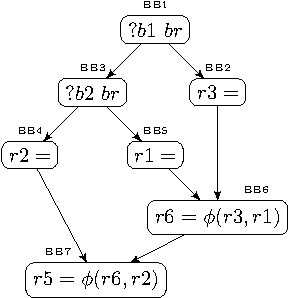
\includegraphics[scale=0.75]{side1.pdf}
    \label{fig:side1}}
  \subfigure[After duplication] {
    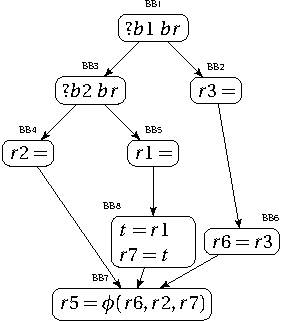
\includegraphics[scale=0.75]{side2.pdf}
    \label{fig:side2}}
  \subfigure[sub-region 1] {
    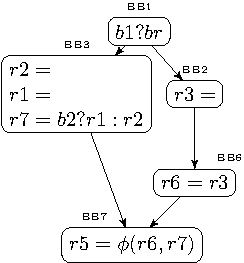
\includegraphics[scale=0.75]{side3.pdf}
    \label{fig:side3}}
  \subfigure[sub-region 2] {
    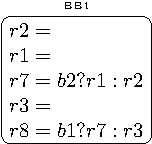
\includegraphics[scale=0.75]{side4.pdf}
    \label{fig:side3}}
\caption{Side entry removal using block duplication}
\label{fig:bbdup}
\end{figure}
\section{Global Framework}

Several algorithmic or design choices impact the effectiveness of if-conversion. As an optimization, the region to if-convert, e.g hyperblock, must be just large enough to have the largest scope of scheduling framework, but in the same time it must not over-commit the machine resources (registers, CPUs). On the contrary, although if-conversion removes branches, I also add some overhead (new instructions to merge predicates, register pressure for speculative conditional, bigger dependence height because of the presence of new data dependencies on the predicates). The newly formed basic block doesn't have a higher schedule estimation than the one that would have been taken if the code was not if-converted.

For this reason, existing approaches of if-conversion are either limitted to a single conditional branch using peepholes style of pattern matching, intrinsic functions (conditional code is inlined by the compiler in the internal representation), or scoping larger but restricted regions such as loops hyperblocks. Such approaches require that the region is isolated from the rest of the control flow, , and more important requires a complicated estimation of the future if-converted region. So many factor impact this (predicate computation, register pressure, dependence height) that the objective function needs to be very conservative. Traditionally if-conversion cover the following steps:

\subsection{Profile support for if-conversion}

2 constraints:
- resource usage/consumption/overcommit
- schedule length
\subsection{SSA Iterative if-conversion}

If you consider the control flow region from \ref{fig:hyper1} 

Globally, the region to if-convert must be carefuly selected. Because of resource consumption issues, merging different paths together can overcommit the architecture ability to execute in parallel the multiple instructions: The data dependences and register renaming, introduce new register constraints. Moving operantions earlier in the instruction stream increase liveranges. 
Another pitfall is to increase the critical path by merging long latencies operation from a less frequenly executed path, thus moving to the critical paths more instructions than the parallelism could absorb.
Finally, for each basic block considered into the region, a predicate must be computed and assigned to the corresponding instructions. Those predicate computation introduce new instructions and new data dependencies.

Conventional if-conversion algorithm should:

\begin{itemize}
\item Isolate the control flow region for which if-conversion is beneficial, using predictive heuristics. Using tail duplication to remove incoming edges. 
\item then for the whole region, Compute and assign a predicate to each basic block.
\item Convert the instructions into predicated ones using the predicate computed from the basic block, and merge the basic blocks.
\item Apply some predicate reduction mechanism to simplify predicate equations.
\item Finally emit the newly predicate computations and the predicated code. If the ISA is not fully predicated, an additional pass is needed to conditionalize them using conditional moves only.
\end{itemize}

In contrast, Using SSA iterative based if-conversion, \ref{fig:hyper1} all those steps become implicit, during the iterative SSA, Since the objective function has a finer granularity. On the case obove, the algorithm will proceed the conditioan absic blocs in postorder.
so first considering the region from {BB4,BB5,BB6} BB5 can be promoted to BB4, and the branch to BB6 becomes r\&q. This remove a branch from BB5 to BB6.
Then second, the region {BB2,BB3 is considered}. Then the region composed of {BB1,and BB2-3}. Finally the hyperblock was naturally formed.

All those operations make the if-conversion process a complex optimization, forcing designers to be extremely conservative, as the objective functions must contain variables not known at the start of the transformation. (such as the complexity of the predicate equations) since moving multiple control paths together can easily exceed processors resources (leading to excessive register pressure) or move infrequently used expensive instruction (memory loads) into the critical path. 

Set of transformations are applied iteratively and aggressively in postorder of the CFG
Start from first inner regions of basic blocks with a single conditional entry
Blocks reached on multiple conditions are detected (predicate merge)
Side entries removed using block duplication 
Decision to continue reconsidered for each region. ``The whole doesn't' exeed the sum of the parts''' or when hazardeous instructions

The process becomes a succession of local decisions, rather than a global decision. And can stop at anytime when the profitability of convertig a subnest is not established, or if a basic block has hazards. At this time, the decsion to stop to to proceed with tail duplication can be taken.

These operation are performed iterativelly on post order, consequently one of the propriety of the algorithms is that psi can be predicated. A Partial out of SSA can be iteratively performed on those regions by removing the $\phi$s and maintening a correct SSA internal representation. The algorithm takes SSA as input and produces SSA if a select instruction is available or $\psi$-SSA if predicated instructions are available. 

\subsection{Hyperblocks}

Traditional framework of if-conversion use Hperblocks as the basic predicated region formation. \cite{Mahlke:1992:ECS:144965.144998}. A hyperblock is a region of code with a single entry and possible, multiple exits where inner branches have been removed thru if-conversion. Tail duplication is used to exclude from the Hyperblock basic blocks, either because the contain hazardeous instructions, or because heuristic decision. 
Traditional hyperblocks formation algorithm create the hyperblocks in the following steps:
\begin{itemize}
\item Create a trace and block selection. A trace is a sequence of basic blocks that can be scheduled together. 
\item Remove side entries with tail duplication, This steps removes scheduling constraints imposed by side entries, or allow regions to be if-converted despite hazards.
\item Finally, if-conversion can be performed to form the hyperblock. 
\end{itemize}

As an example of hyperblock formation, consider the example \ref{fig:hyper1}. This loop containts two branches, and so if-converting it would be profitable. However, block selection has excluded BB2. and had integrated BB5, because heuristics have determined that the schedule of BB5 inside BB4 would be beneficial. The hyperblock containts {BB1, BB3, BB4, BB5, BB6}. Since BB4 is has side entry, it must be removed by tail duplication. \ref{fig:hyper2} shows the  control flow after block duplication. Notice that a new node, BB7, have been added after the tail duplication by a process called branch coalescing. Finally \ref{fig:hyper3} shows the code once if-converted.
\begin{figure}[h]
  \subfigure[loop] {
    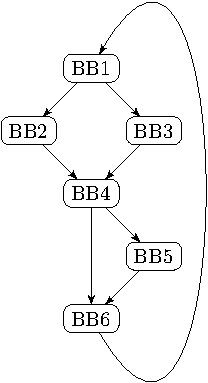
\includegraphics[scale=0.7]{hyper1.pdf}
    \label{fig:hyper1}}
  \subfigure[standard tail-duplication] {
    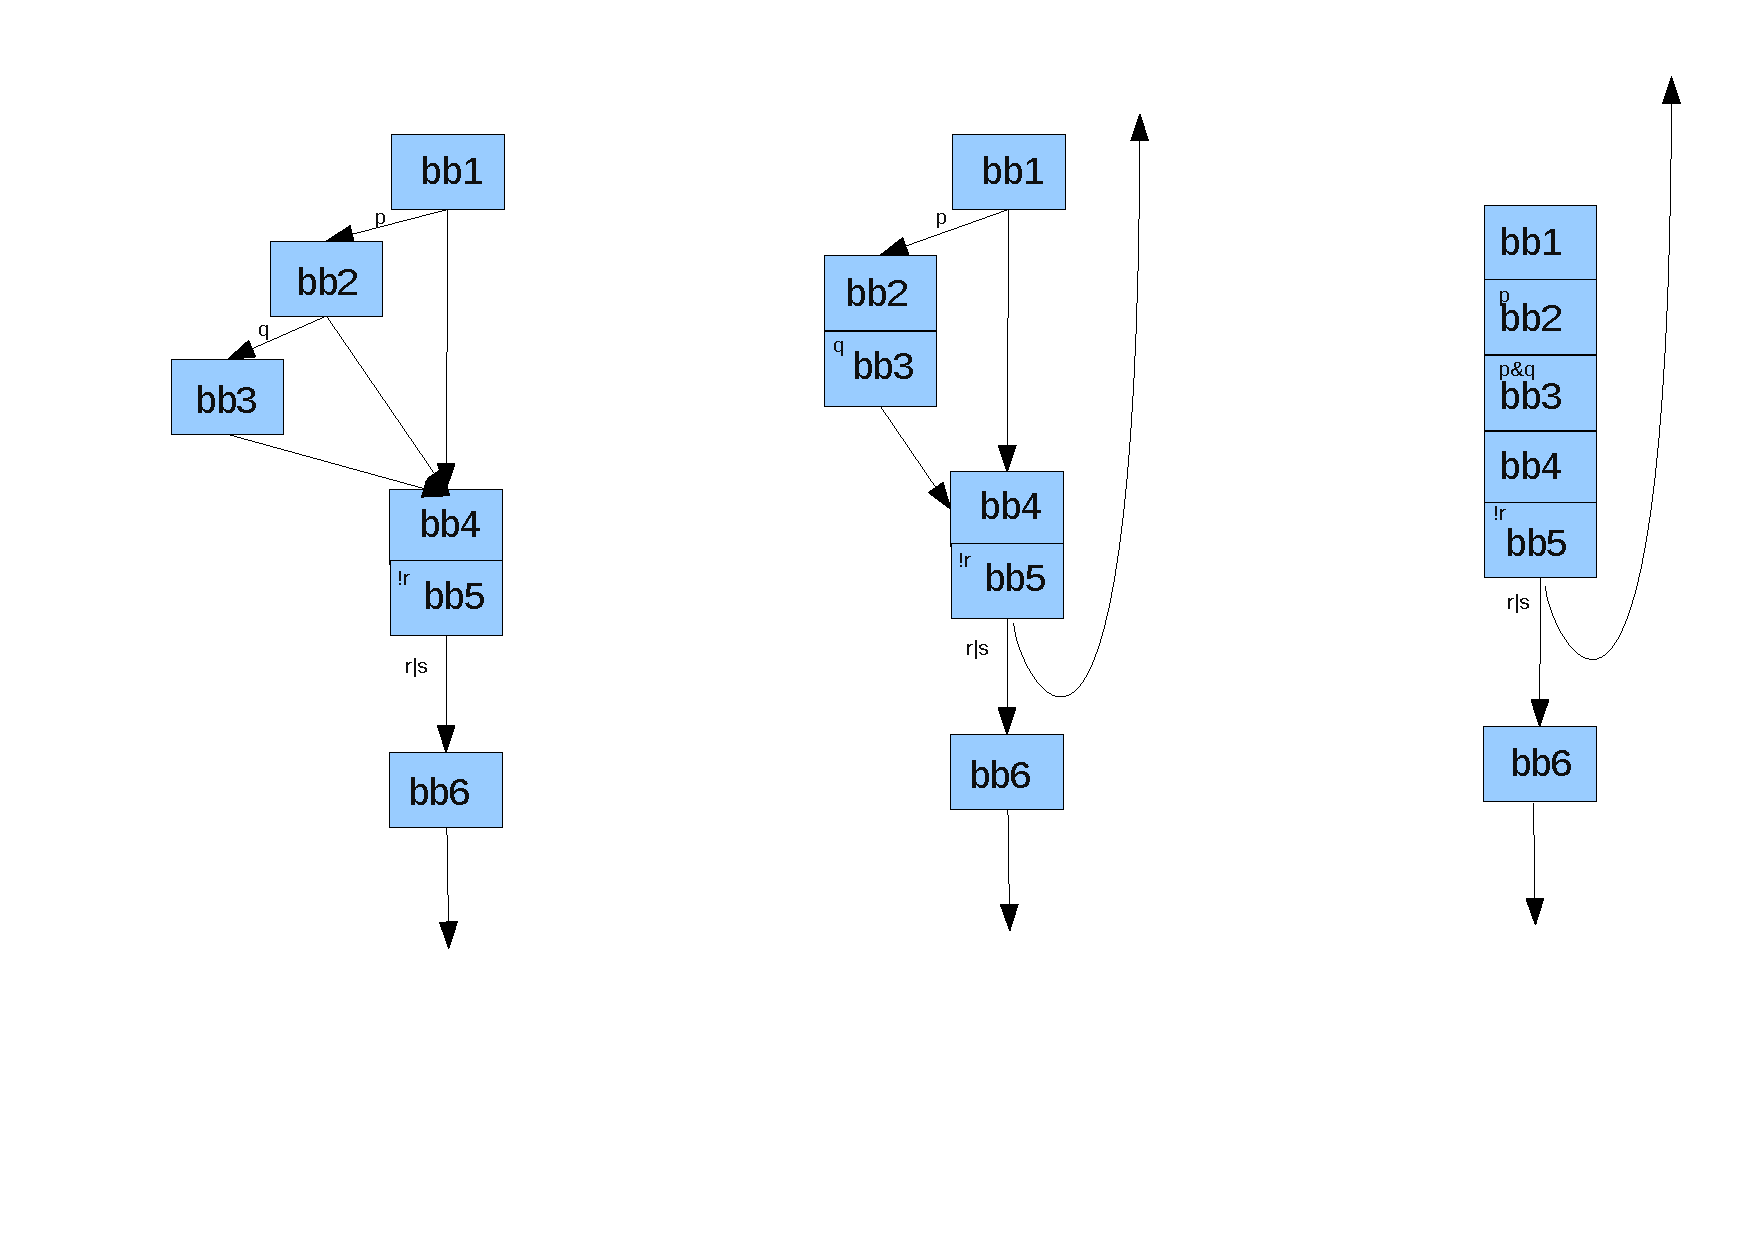
\includegraphics[scale=0.7]{hyper2.pdf}
    \label{fig:hyper2}}
  \subfigure[after SSA if-conversion] {
    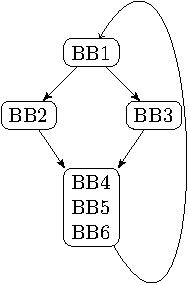
\includegraphics[scale=0.7]{hyper4.pdf}
    \label{fig:hyper4}}
  \subfigure[final flow] {
    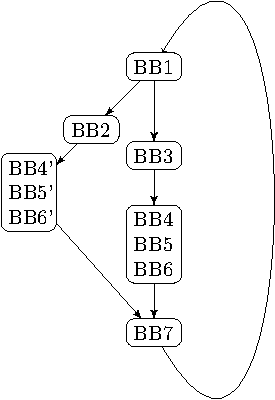
\includegraphics[scale=0.7]{hyper3.pdf}
    \label{fig:hyper3}}
\end{figure}
The fact that the if-conversion happens after tail-duplication. In the resulting code happens to be difficult to schedule efficiently, over committing resources. Hyperblock formation, if-conversion and speculation introduce a major phase ordering problem. A technique called ``Reverse If-Conversion'' \cite{August:1999:PRI:326224.325595} overcomes this problem, allowing to use aggressive if-conversion framework and reconstructing the control flow at schedule time.

Consider in contrast how tail-duplication is performed in a lazy way, after the code have been if-converted. \ref{hyper4} shows the same loop body were the second $if$ region have been SSA if-converted. The decision to if-convert the region formed by {BB1, BB2, BB3} is now local and can be taken conservatively. Only at this stage, if necessary, tail-duplication can be performed to remove the side entry coming from BB2. Duplicating a single predicated block is now a very simple operation.

\section{Conclusion}
Both benefits, increase speculation to extract ILP, while leveraging on predicated possibilities to remove branches.
Hyperblock formation is more conservative, critical path is easier to calculate, removing the need for reverse-if-conversion. Only control flow dependencies between a confluent point, a definition and the definition of the predicate is considered. 
Easier to calculate beneficial optimisation locally and reconsider for each sub-region as the hyperblock grows, rather that globaly and reverse if-conversion
Only variables that join need to be conditionaliez, other can be speciulated if possible, reducing predicate dependencies

Speculated model: enter in strict SSA and produces strict SSA
Predicated model enter ins strict SSA and produces psi SSA.



